% Mid-term check report (CSCI-B590, due Nov 13, 2026). DRAFT, kept up to date as results come in.
% Build: tectonic report/midterm.tex   (or pdflatex). Figures: python -m scripts.report_figs
\documentclass[conference]{IEEEtran}
\usepackage[T1]{fontenc} % Times text with real bold/italic under Tectonic (TU encoding has no ptm)
\usepackage{amsmath,amssymb}
\usepackage{graphicx}
\usepackage{booktabs}
\usepackage{xcolor}
\usepackage{tikz}
\usetikzlibrary{arrows.meta,positioning,fit}
\usepackage[hidelinks]{hyperref}
\graphicspath{{figs/}}
\newcommand{\todo}[1]{\textcolor{red}{[#1]}}

\begin{document}
\title{APF-Shielded Deep RL for Autonomous Racing:\\Mid-term Report}

\author{\IEEEauthorblockN{Christine Chen}
\IEEEauthorblockA{\textit{Luddy School of Informatics,}\\ \textit{Computing, and Engineering}\\
Indiana University Bloomington\\ cch8@iu.edu}
\and
\IEEEauthorblockN{Chinmay Deshpande}
\IEEEauthorblockA{\textit{Luddy School of Informatics,}\\ \textit{Computing, and Engineering}\\
Indiana University Bloomington\\ chidesh@iu.edu}
\and
\IEEEauthorblockN{Gabriel Shores}
\IEEEauthorblockA{\textit{Luddy School of Informatics,}\\ \textit{Computing, and Engineering}\\
Indiana University Bloomington\\ gshores@iu.edu}}

\maketitle

\begin{abstract}
We race a PPO agent against three PID and Pure Pursuit opponents in F1TENTH Gym, with an artificial potential
field (APF) acting as a safety shield that intervenes only when the agent's own action is predicted to cause a
crash. The full pipeline now runs end to end: track, opponents, classical baselines, shielded and unshielded PPO
with the three-stage curriculum, and a race-day evaluation with all six proposed metrics. Following the proposal
feedback, the shield is action-conditioned rather than additive, the simulator has friction-limited tyres, and
every metric has a target. On the shared race seeds our agent finishes 43 of 50 five-lap races (PID+APF: 28,
$p=0.002$), laps 8\,s faster than PID+APF, crashes about 10$\times$ less often during training than unshielded
PPO, and meets all six metric targets on the 20-race protocol. The main open problem is variance across training
seeds; a residual policy trained with the shield removes most of it (81\% of 150 races finished over three
seeds, PID+APF 56\%) and is our final controller.
\end{abstract}

\section{Introduction}
Classical racing controllers such as PID steering with an APF avoidance layer are safe but slow near obstacles and
cannot plan a pass; deep RL learns fast lines and tactics but crashes constantly while learning and gives no safety
guarantee. Our goal is to combine them: a PPO agent races, and an APF shield steps in only when a crash is
imminent, with a reward penalty for every intervention.

\textbf{Updated scope.} Four changes since the proposal, three of them prompted by the feedback:
(1) The additive, clipped APF of the proposal's Eq.~2--3 cannot prevent violations, and its weight $w(d)$ ignores
the agent's action. We confirmed both experimentally (Sec.~\ref{sec:results}) and replaced it with an
\emph{action-conditioned} shield that simulates the agent's action and only intervenes if that action is predicted
unsafe; Eq.~2--3 is kept as a baseline. (2) Stock F1TENTH tyres have no grip limit (we measured 2.4\,g of lateral
acceleration at $\mu = 1.05$), so we added a friction-circle tyre model and traction control; this also makes the
``grip left over after cornering'' reach physically meaningful. (3) Training efficiency is measured with the shield
removed, and crashes during training are reported, because a shield trivially keeps laps clean. (4) We added a
ResRace-style residual policy~\cite{zhang2022} as a baseline to make the difference from ResRace and
RaceMOP~\cite{trumpp2024} testable.

\textbf{Contribution.} In ResRace and RaceMOP the APF shapes every command; in ours the policy drives and the APF
acts only when an exact-model rollout of the policy's own action predicts a collision or loss of control (3\% of
race steps for training seed 0), with a fallback manoeuvre when no corrected action is safe.

\textbf{What works now.} Everything in the proposal's plan through ``race day'': the Singapore-inspired track
(199\,m, 2.8\,m wide), three opponents, Pure Pursuit and PID+APF baselines, PPO with and without the shield on
three training seeds each, the four-car race evaluation (20 shared seeds, 5 laps, nominal and randomised), all six
metrics with targets and Mann--Whitney U tests, g-g and telemetry plots, and race videos. The code, a log of every
run and 33 documented problems are in the team repository.

\section{System Architecture}
\begin{figure}[t]
\centering
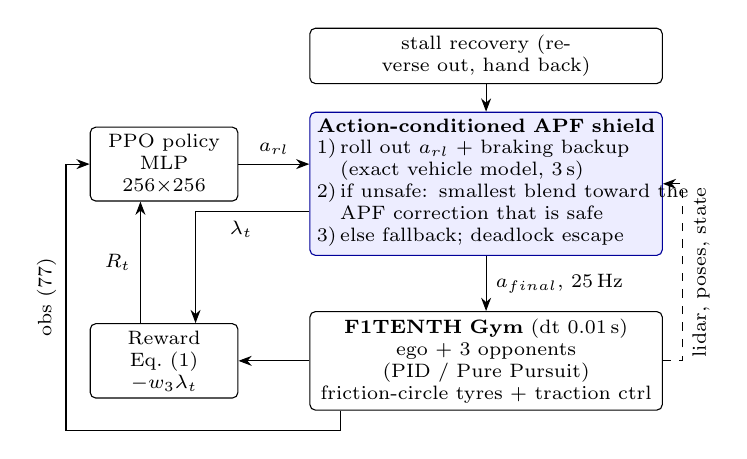
\begin{tikzpicture}[font=\scriptsize, >=Stealth,
  box/.style={draw, rounded corners=2pt, align=center, inner sep=2.5pt, fill=white},
  hl/.style={box, fill=blue!7, draw=blue!60!black}]
\node[hl, text width=43mm] (sh) at (0,0) {\textbf{Action-conditioned APF shield}\\[0.3mm]
  \begin{tabular}{@{}l@{\,}l@{}}
  1) & roll out $a_{rl}$ + braking backup\\ & (exact vehicle model, 3\,s)\\
  2) & if unsafe: smallest blend toward the\\ & APF correction that is safe\\
  3) & else fallback; deadlock escape
  \end{tabular}};
\node[box, text width=43mm, above=3.5mm of sh] (rec) {stall recovery (reverse out, hand back)};
\node[box, text width=43mm, below=7mm of sh] (sim) {\textbf{F1TENTH Gym} (dt 0.01\,s)\\
  ego + 3 opponents (PID / Pure Pursuit)\\ friction-circle tyres + traction ctrl};
\node[box, text width=17mm, left=9mm of sh.west, anchor=east, yshift=2.5mm] (ppo) {PPO policy\\MLP $256{\times}256$};
\node[box, text width=17mm, anchor=east] (rew) at (ppo.east |- sim.center) {Reward Eq.~(1)\\$-w_3\lambda_t$};
% policy -> shield -> simulator
\draw[->] (ppo.east) -- node[above]{$a_{rl}$} (ppo.east -| sh.west);
\draw[->] (sh) -- node[right]{$a_{final}$, 25\,Hz} (sim);
\draw[->] (rec) -- (sh);
% shield intervention -> reward; reward -> policy
\draw[->] ([yshift=-3.5mm]sh.west) -| node[pos=0.3, below]{$\lambda_t$} ([xshift=4mm]rew.north);
\draw[->] ([xshift=-3mm]rew.north) -- node[left]{$R_t$} ([xshift=-3mm]ppo.south);
% simulator -> reward and observation -> policy
\draw[->] (sim.west) -- (rew.east);
\coordinate (oa) at ([xshift=4mm, yshift=-2.5mm]sim.south west);
\coordinate (ob) at ([xshift=-3mm]rew.west |- oa);
\draw[->] ([xshift=4mm]sim.south west) -- (oa) -- (ob) -- node[pos=0.5, above, sloped]{obs (77)} (ob |- ppo.west)
  -- (ppo.west);
% sensing used by the shield
\draw[->, dashed] (sim.east) -- ++(2.5mm,0) |- node[pos=0.25, below, sloped]{lidar, poses, state} (sh.east);
\end{tikzpicture}
\caption{Control loop. The shield is part of the environment, so it can be switched off without touching the
policy; it reports its intervention strength $\lambda_t$ to the reward and the metrics.}
\label{fig:arch}
\end{figure}

Fig.~\ref{fig:arch} shows the loop. At 25\,Hz the policy maps a 77-value observation to an action; the shield
checks it against the lidar scan (every third of the 1080 beams), the known track walls and the opponents' poses, and passes on
either the action itself or a corrected one. The simulator integrates the dynamic single-track model with RK4 at
0.01\,s for all four cars. Opponents alternate PID (curvature feed-forward plus PID on cross-track error) and Pure
Pursuit at 50--75\% of a grip-limited speed profile, with gap keeping. We patched F1TENTH Gym's lidar ray casting
(about 10$\times$ faster, $\sim$400 control steps/s per core without the shield), and training runs 7
environments in parallel on a laptop CPU (3.5\,M steps in about 2\,h).

\section{Implemented Approach}
\subsection{Vehicle model}
F1TENTH default parameters (3.74\,kg, wheelbase 0.33\,m, $\mu = 1.0489$). Each axle's lateral force is capped by a
friction circle, $|F_y| \le \sqrt{(\mu F_z)^2 - (F_z a_x/g)^2}$, identical to the stock model below the limit;
traction control clamps the speed loop's acceleration to $\sqrt{(0.95\mu g)^2 - (v r)^2}$. This closes the
sliding exploit reported by Evans et al.~\cite{evans2023}.

\subsection{Reinforcement learning agent}
\textbf{Observation:} 60 min-pooled lidar sectors, speed, yaw rate, steering angle, lateral offset and heading
error, the two nearest opponents (relative position and velocity), and the previous action.
\textbf{Action:} steering in $\pm0.42$\,rad and target speed in 1--16\,m/s. \textbf{Reward} (proposal Eq.~1):
\begin{equation}
R_t = w_1 v_\parallel + w_2 \Delta s + w_5 \mathbb{1}_{pass} - w_3 \lambda_t - w_4 \mathbb{1}_{collision}
\end{equation}
with $(w_1,w_2,w_3,w_4,w_5) = (0.002, 0.1, 0.1, 10, 2)$; a pass counts once the ego holds a lead of one car
length for 2\,s without contact. Episodes last 40\,s and end on any collision.
\textbf{PPO} (Stable-Baselines3): lr $3\!\times\!10^{-4}$, 7 envs $\times$ 512 steps, batch 1024, 10 epochs,
$\gamma = 0.99$, GAE 0.95, clip 0.2. \textbf{Curriculum:} solo laps (1.5\,M steps), slow opponents (1\,M),
opponents at varied speeds and start gaps (1\,M), with friction $\times U(0.85, 1.15)$ and lidar noise up to
5\,cm randomised per episode. The unshielded ablation uses the same curriculum with the shield off in every stage.

\subsection{APF shield}
\textbf{Field.} For beam $i$ at angle $\theta_i$ with clearance $c_i$ from the car outline, the influence distance
is the braking distance on the closing speed, and each beam adds a repulsive force:
\begin{gather}
\begin{gathered}
d_{0,i} = d_{min} + \frac{\max(v\cos\theta_i, 0)^2}{2 a_b},\\
\rho_i = \mathrm{clip}\!\left(\frac{d_{0,i} - c_i}{d_{0,i} - d_{crit}}, 0, 1\right),
\end{gathered}\\
\mathbf{F} = -\textstyle\sum_i \rho_i^2\, \Delta\theta \,(\cos\theta_i, \sin\theta_i),
\end{gather}
where $a_b = \sqrt{(\mu g)^2 - (v r)^2}$ is the grip left after cornering (``grip reach''; a fixed 6\,m/s$^2$
is the alternative). Opponents add an elliptical field stretched along their heading. The lateral force becomes a
steering correction and the backward force a speed reduction, giving the corrected action $a_{corr}$.

\textbf{Action-conditioned decision.} Let $C(a)$ be the minimum clearance of the car's three covering circles to
lidar points, map walls and opponents (assumed to brake at 6\,m/s$^2$) over a rollout that holds $a$ for one
control step and then brakes while holding the lane, using the simulator's own vehicle model (verified to
$<2$\,cm); $C(a) = -1$ if the predicted body slip exceeds 20$^\circ$. Then
\begin{equation}
a_{final} =
\begin{cases}
a_{rl} & C(a_{rl}) \ge c_{safe}\\
(1-\lambda) a_{rl} + \lambda a_{corr} & \text{smallest safe } \lambda \in \Lambda\\
\text{fallback} & \text{otherwise,}
\end{cases}
\end{equation}
with $\Lambda = \{\tfrac14,\tfrac12,\tfrac34,1\}$ and $c_{safe} = 5$\,cm. The fallback is the braking backup itself (which keeps the check recursively feasible)
or the safest of seven other braking manoeuvres. Two additions came from failures we observed on race day:
a \emph{deadlock escape} (when stopped inside the margin, allow 2\,cm of clearance loss and slow creep or reverse
manoeuvres) and a \emph{stall recovery} (if the car stops nose-to-wall, reverse with the steering that turns the
nose back to the track, then hand control back); both are filtered by the shield.

\subsection{Baselines}
Pure Pursuit on the centerline; PID+APF with the proposal's additive Eq.~2--3 (gains grid-searched for this
track); unshielded PPO; PPO trained with the additive Eq.~2--3 shield; and a ResRace-style residual policy
(action = PID+APF action $+\,0.3\times$ policy).

\section{Preliminary Results}\label{sec:results}
\textbf{Shield without learning.} With friction-circle tyres, scripted bad drivers (too fast, ignoring traffic,
random) crash in 100\% of trials with no shield \emph{and} with the additive Eq.~2--3 shield; with the
action-conditioned shield and fallback, 0/12/0\% with fixed reach and 0/38/12\% with grip reach (used by the
agent). On stock tyres the additive shield is active on 98\% of steps for a too-fast driver, ours on 18\%.

\textbf{Training safety} (Fig.~\ref{fig:train}). Over 3.5\,M steps the shielded agent crashed in 96--313
episodes versus 2295--2769 without the shield (3 seeds each); PPO trained with the additive shield crashed
1786--2333 times (3 seeds), hardly better than none. Before its first clean lap the shielded agent crashed 8--11 times versus 969--1080.
With the shield \emph{removed} for the measurement, both variants complete their first clean solo lap after
150--200\,k steps, so the shield made training far safer but not faster at learning to lap. The final
controller's recipe (residual policy trained with our shield) is both: 81--133 crashes in all of training and a first
solo lap under 34\,s (faster than any classical lap) after 200--250\,k steps, versus 450--800\,k for PPO with our
shield and 550--850\,k without.

\begin{figure}[t]
\centering
\includegraphics[width=\columnwidth]{training_crashes.pdf}
\caption{Cumulative crashes during training. Each line is one training seed.}
\label{fig:train}
\end{figure}

\begin{table}[t]
\caption{Race day, training seed 0, nominal conditions (5 laps, 3 opponents, DNF on first collision).
Lap: mean clean lap. Coll.: collisions per 10 laps. 50 races: finished on 50 shared seeds, nominal / randomised.}
\label{tab:race}
\centering
\footnotesize
\setlength{\tabcolsep}{3pt}
\begin{tabular}{lccccc}
\toprule
Controller & Fin./20 & Lap (s) & Coll. & Passes & 50 races\\
\midrule
\textbf{PPO + our shield} & \textbf{19} & 34.7 & \textbf{0.10} & 3.15 & \textbf{43} / 35\\
Residual PPO trained w/ shield & 15 & 32.1 & 0.59 & 3.15 & 39 / \textbf{37}\\
PPO + additive APF (Eq.~2--3) & 18 & 47.6 & 0.21 & 0.85 & 39 / 34\\
PID + APF & 12 & 42.8 & 1.09 & 1.35 & 28 / 25\\
Residual PPO (ResRace-style) & 10 & \textbf{30.4} & 1.60 & 2.20 & --\\
PPO, no shield & 0 & 32.5 & 7.35 & 1.35 & --\\
Pure Pursuit & 0 & -- & 61.4 & 0 & --\\
\bottomrule
\end{tabular}
\end{table}

\begin{figure}[t]
\centering
\includegraphics[width=\columnwidth]{tradeoff.pdf}
\caption{Safety versus speed (Table~\ref{tab:race}); marker size grows with races finished.}
\label{fig:tradeoff}
\end{figure}

\textbf{Race day} (Table~\ref{tab:race}, Fig.~\ref{fig:tradeoff}). On 50 shared race seeds our agent finishes
more races than PID+APF ($p = 0.002$ nominal, Fisher; $p = 0.07$ randomised) while lapping 8\,s faster; against the additive-shield agent the
finish rates are statistically tied ($p = 0.44$), but ours laps 12\,s faster with 2.7$\times$ the passes over 50 races
($p \approx 10^{-8}$, Mann--Whitney), the timid behaviour the proposal predicted for an always-on APF. On the 20 seed-0 races our agent meets all
six metric targets in both conditions: lap time 0.81$\times$ PID+APF ($\le$\,0.95), 0.10 / 0.47 collisions per 10 laps
($\le$\,0.5), 85\% overtake success ($\ge$\,70\%), shield active on 3\% of steps ($\le$\,10\%), 17\% of time above
90\% of $\mu g$ ($\ge$\,10\%) and 0.0\% above 15$^\circ$ slip ($\le$\,1\%). Over all 50 races the randomised
collision rate is 0.77, which misses its target. Adding our shield to the residual
policy only at race time fails (2--4 of 20 finished, deadlocks and slides), but training the residual policy with
the shield works: statistically tied with ours on finishes over 50 races ($p = 0.44$ / $0.82$) and
1.9--2.5\,s per lap faster on all three training seeds (39--42 of 50 finished nominal, 37--40 randomised).

\textbf{Across training seeds} the results vary a lot (Fig.~\ref{fig:seeds}). With the final shield, seeds 0 and 2 finish 19/20 and seed 1
only 1/20 (13.0\,$\pm$\,8.5, mean $\pm$ population s.d.\ over 3 seeds), versus 3.0\,$\pm$\,2.4 without a shield; collisions per 10 laps are
1.63\,$\pm$\,2.16 versus 4.38\,$\pm$\,2.12. Seed 1 learned to drive at the limit: replaying a crash shows the
predicted clearance shrinking for several steps while staying above the 5\,cm margin, after which every braking
manoeuvre is predicted to spin. Fig.~\ref{fig:fail} shows where races end: most failures of the shielded agent
were in the tight 2.5\,m-radius corners at 84--126\,m, where the policy stalled with its nose against the wall; the stall recovery removed
most of them. \textbf{A fix for the sliding seed:} retraining seed 1 with a slip penalty
$w_6 \max(|\beta| - 0.15, 0)$ added to Eq.~(1) ($w_6 = 1$, final shield from the start) gives 18/20 finished with the stall
recovery (17/20 randomised), 0.11 collisions per 10 laps and 32.5\,s laps. It is not a general fix: seeds 0 and 2 with
the same recipe finish only 11/20 (13.3\,$\pm$\,3.3 over three seeds). The residual policy trained with the shield is more
consistent: over three seeds it finishes 16.0\,$\pm$\,0.8 of 20 races (16.7\,$\pm$\,0.5 randomised), with
0.47\,$\pm$\,0.10 collisions per 10 laps and 32.2\,$\pm$\,0.1\,s laps, never stuck. \textbf{We therefore adopt it as
the final controller.} Pooled over 150 races it meets five of six targets (lap 0.76$\times$ PID+APF, 0.43
collisions per 10 laps, 91\% overtake success, shield on 5\% of steps, 0\% slip) and misses the grip target
(8.8\% of time above 90\% of $\mu g$). The g-g diagrams (Fig.~\ref{fig:grip}) show that this target measures the
wrong thing: plain PPO reaches 35\% with a bang-bang throttle (31\% of the race braking and 30\% accelerating
harder than $0.5\mu g$, clipped by traction control at $\pm0.95\mu g$) but corners above $0.6\mu g$ only 5\% of the
time, like PID+APF. The final controller corners that hard 14\% of the time and brakes hard half as often, which is
where its 6\,s per lap come from. We will report cornering grip instead.

\begin{figure}[t]
\centering
\includegraphics[width=\columnwidth]{failure_map.pdf}
\caption{Where races end on the lap (3 training seeds, nominal and randomised races pooled).}
\label{fig:fail}
\end{figure}

\begin{figure}[t]
\centering
\includegraphics[width=\columnwidth]{seed_spread.pdf}
\caption{Races finished out of 20 per training seed (filled: nominal, hollow: randomised; dashed: PID+APF).
The residual policy trained with our shield has the smallest spread; plain PPO with our shield has both the
best and the worst seed.}
\label{fig:seeds}
\end{figure}

\begin{figure}[t]
\centering
\includegraphics[width=\columnwidth]{grip_use.pdf}
\caption{g-g diagrams, nominal races, all training seeds (circle: friction limit). Corner: time with lateral
acceleration above $0.6\mu g$; brake: braking harder than $0.5\mu g$ (dotted lines).}
\label{fig:grip}
\end{figure}

\textbf{Our shield, or any shield?} Trained with the additive Eq.~2--3 shield instead of ours, the residual
policy fails (0--1 of 20 finished on two seeds; 2.1$\times$ the training crashes of PPO with no shield). With the
policy output fixed at zero, PID+APF plus the additive shield already finishes 0/20: the residual base has its own
APF, and the two fields stack. Our shield, which leaves safe actions alone, composes: PID+APF plus our shield with
no learning finishes 20/20 without a collision (16/20 randomised) but laps at 42.5\,s. The learned residual buys
10\,s per lap on top of it.

\textbf{What still fails.} 60 of the final controller's 62 non-finishes in 300 races are contacts with opponents.
Of seed 0's 24, 15 are the ego cutting back in front of a car it has just passed. The shield's prediction lets every opponent
brake at 6\,m/s$^2$, the worst case for a car ahead but the best case for a car just passed, which keeps its speed.
Checking both (brake or hold speed) cuts car contacts from 60 to 25 ($p = 6\cdot10^{-5}$) but adds
15 wall hits when nothing is safe under both. Falling back to braking-only then gives 256 of 300 finished (238
before), 38 car contacts and 4 wall hits. With the friction estimate below as well, 269 of 300
finish ($p = 7\cdot10^{-4}$) with 30 car contacts and no wall hit, 0.5\,s per lap slower.

\textbf{Outside the training friction.} At friction $\times$0.8 (trained on 0.85--1.15) the final controller
finishes 52\% of races, PID+APF 50\%, PPO + shield 85\%. With the shield told the true friction it finishes 83\%
($p = 4\cdot10^{-4}$). At $\times$0.7 the true friction lifts it from 27\% to 67\% and PPO from 35\% to 90\%, so
the friction model is the weak point. Estimating it online from tyre saturation gives 90\% at $\times$0.8 and,
smoothed, 78\% at $\times$0.7 at no cost in normal races. With one opponent all controllers finish 85--100\%, with five PID+APF
48\% and ours 77\%.

\textbf{Why the tyre model matters.} On stock tyres the same recipe laps 5\,s faster by cornering above the
friction limit 9.7\% of the time; with ours, 0\%.

\textbf{Generalisation.} On a second track that no policy saw in training (228\,m, a 55\,m straight, a fast
sweeper and a 2.5\,m hairpin; 20 races), the final controller finishes 18.3 of 20 over three seeds (16.3 randomised) in
31.2\,s with 3.8 passes per race, against PID+APF 15/20 in 39.3\,s. Plain PPO + shield finishes 16.7 (14.0, one
seed 5/20) in 37.5\,s, PPO without a shield 1/20.

\textbf{Negative results.} A lower intervention penalty ($w_3 = 0.02$) let the agent hand braking to the
shield (35\% of steps) and deadlock. Shield dropout gave a policy that is safe with no shield (16/20) but timid
(0.25 passes per race). A wider residual (scale 0.5) helped one seed (19/20) and let the other slide (14/20).

\section{Plan to the Final Demo}
\textbf{Remaining tasks and milestones} (final demo December 7):
\begin{itemize}
\item \emph{Nov 13--20:} retrain the policy with the improved shield (running); report cornering grip instead of
the grip target.
\item \emph{Nov 21--27:} test the three-seed baselines on both tracks; stress tests of the final shield (friction,
number of opponents).
\item \emph{Nov 28--Dec 3:} freeze the code; run the final evaluation (all controllers, 3 training seeds, 50 race
seeds, nominal and randomised); telemetry, g-g diagrams and videos.
\item \emph{Dec 4--7:} final report, presentation and live demo (recorded four-car races).
\end{itemize}
\textbf{Evaluation plan.} Controllers: Pure Pursuit, PID+APF, unshielded PPO, PPO with the additive Eq.~2--3
shield, ResRace-style residual PPO (with and without our shield) and ours. Scenarios: five-lap four-car races on
50 shared seeds, nominal and randomised, three training seeds per learned controller, and the stress tests.
Metrics: the six targets (cornering grip in place of time above 90\% of $\mu g$), races finished, crashes in
training and steps to the first fast lap. Tests: Fisher's exact test on finish rates, Mann--Whitney U
on per-race values.

\textbf{Team roles.} \todo{Team: fill in who owns which part (e.g., simulator and track, shield, RL training,
evaluation and analysis).}

\section*{Acknowledgement}
Claude (Anthropic) was used to write and debug code, run experiments, and draft this report. \todo{Team: edit to
match how you used it.}

\begin{thebibliography}{9}
\bibitem{zhang2022} R. Zhang et al., ``Residual policy learning facilitates efficient model-free autonomous
racing,'' \emph{IEEE Robot. Autom. Lett.}, vol.~7, no.~4, pp. 11625--11632, 2022.
\bibitem{trumpp2024} R. Trumpp et al., ``RaceMOP: Mapless online path planning for multi-agent autonomous racing
using residual policy learning,'' in \emph{Proc. IEEE/RSJ IROS}, 2024, pp. 8449--8456.
\bibitem{evans2023} B. D. Evans, H. A. Engelbrecht, and H. W. Jordaan, ``High-speed autonomous racing using
trajectory-aided deep reinforcement learning,'' \emph{IEEE Robot. Autom. Lett.}, vol.~8, no.~9, pp. 5353--5359,
2023.
\end{thebibliography}
\end{document}
